\section[Using the haplo.post.prob() function for Hap-Clustering]{Using the \code{haplo.post.prob()} function for Hap-Clustering}
\label{sec:haplo}
\addcontentsline{toc}{section}{\thesection. Using the \code{haplo.post.prob()}\ function for Hap-Clustering \vspace{-0.3cm}}

Haplotype grouping \citep{tzeng2005} for SNP datasets
can be viewed as an alternative method to phyloclustering.
The author's \proglang{R} code has been integrate into \pkg{phyclust},
and the original function has been renamed \code{haplo.post.prob()}.
The example used by the author is the Crohn's disease dataset
\citep{Hugot2001}, which is also included in the \pkg{phyclust} package.
The original description of the author's \proglang{R} code is in the
install directory 
\url{phyclust/doc/Documents/tzeng-Readme.txt} or in the source code directory
\url{phyclust/inst/doc/Documents/tzeng-Readme.txt}.

The following example returns the same results as \cite{tzeng2005}, where
the predicted number of clusters based on her information criterion is $13$.
The function returns a list object, here stored in \code{ret}.
The list element \code{ret$haplo} stores information about the SNP sequences,
\code{ret$FD.id} and \code{ret$RD.id} store the full and reduced dimensional
indices, 
\code{ret$FD.post} and \code{ret$RD.post} store the full and reduced dimensional
posterior probabilities, and \code{g.truncate} shows
the number of clusters,
the truncated results as described in \cite{tzeng2005}.
\begin{Code}
> data.path <- paste(.libPaths()[1], "/phyclust/data/crohn.phy", sep = "")
> my.snp <- read.phylip.snp(data.path)
> ret <- haplo.post.prob(my.snp$org, ploidy = 1)
> str(ret)
List of 6
 $ haplo     :List of 6
  ..$ haplotype: num [1:39, 1:8] 0 1 1 0 1 1 0 1 1 0 ...
  ..$ hap.prob : num [1:39] 0.00454 0.00181 0.11797 0.00635 0.00635 ...
  ..$ post     : num [1:1102] 1 1 1 1 1 1 1 1 1 1 ...
  ..$ hap1code : int [1:1102] 1 1 1 1 1 2 2 3 3 3 ...
  ..$ hap2code : int [1:1102] 1 1 1 1 1 2 2 3 3 3 ...
  ..$ indx.subj: int [1:1102] 1 2 3 4 5 6 7 8 9 10 ...
 $ FD.id     : int [1:39] 3 9 18 22 27 28 30 31 34 35 ...
 $ RD.id     : int [1:13] 3 9 18 22 27 28 30 31 34 35 ...
 $ FD.post   : num [1:1102, 1:39] 0 0 0 0 0 0 0 1 1 1 ...
 $ RD.post   : num [1:1102, 1:13] 0 0 0 0 0 1 1 1 1 1 ...
 $ g.truncate: int 13
> getcut.fun(sort(ret$haplo$hap.prob, decreasing = TRUE),
>            nn = my.snp$nseq, plot = 1)
\end{Code}

The \code{getcut.fun()} produces a plot based on the information
criterion, which can be used to visualize the truncated dimension.
In Figure~\ref{fig:getcut}, the horizontal line indicates the cut point
of $13$ haplotypes.
\begin{figure}[h]
\begin{center}
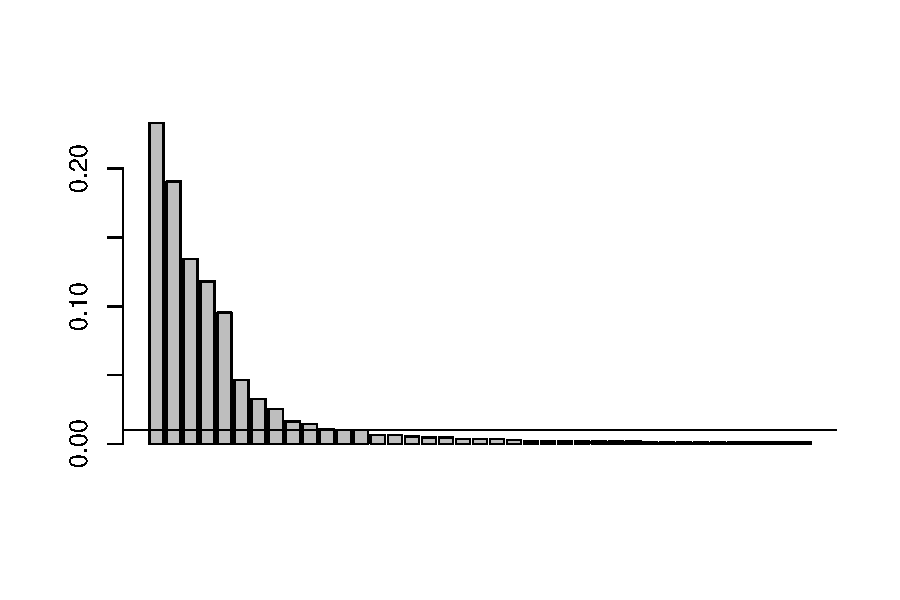
\includegraphics[width=6.0in]{./phyclust-include/f-getcut}
\caption{A getcut plot for the Crohn's disease dataset.}
\label{fig:getcut}
\end{center}
\end{figure}
